\chapter{Das Singulett, Bells Ungleichung und das No-Cloning-Theorem}

\lectureoverview{Ein relatives Minuszeichen macht aus einem lediglich korrelierten Zustand zweier Spins das rotationsinvariante Singulett. Wir identifizieren diesen Zustand, indem wir seinen Gesamtspin berechnen, formulieren mithilfe seiner perfekten Antikorrelation ein Bell-Experiment und übersetzen klassische Aussagen in quantenmechanische Projektionsoperatoren. Die daraus folgenden Wahrscheinlichkeiten verletzen die klassische Zählungleichung von Bell. Fragen zu Lokalität, zum zeitlichen Ablauf der Experimente und zur Unschärfe führen dann zu einer zweiten Konsequenz der linearen Quantenmechanik: Ein unbekannter Zustand kann nicht mit einer universellen Klonmaschine kopiert werden.}

\section{Welchen Unterschied kann ein Vorzeichen machen?}

Betrachten wir zwei Elektronen und lassen in den Basiszuständen das Tensorproduktsymbol weg:
\begin{equation}
  \ket{ud}\equiv\ket{u}_1\otimes\ket{d}_2,
  \qquad
  \ket{du}\equiv\ket{d}_1\otimes\ket{u}_2.
\end{equation}
Zwei besonders einfache Superpositionen unterscheiden sich nur durch ein Vorzeichen,
\begin{equation}
  \ket{\psi_\pm}
  =
  \frac{\ket{ud}\pm\ket{du}}{\sqrt2}.
  \label{eq:l05-two-signs}
\end{equation}
Der Faktor \(1/\sqrt2\) sorgt dafür, dass die Gesamtwahrscheinlichkeit eins ist. In beiden Zuständen liefert eine Messung entlang der dritten Achse entgegengesetzte Ergebnisse: Ist Elektron 1 spinaufwärts, so ist Elektron 2 spinabwärts, und umgekehrt. Allein anhand dieser Korrelation lässt sich das Vorzeichen daher nicht feststellen. Dennoch sind die beiden Zustände physikalisch verschieden.

Bei den Rechnungen werden wir wiederholt die Wirkungen der Pauli-Matrizen verwenden:
\begin{align}
  \sigma_1\ket{u}&=\ket{d},&
  \sigma_1\ket{d}&=\ket{u},\nonumber\\
  \sigma_2\ket{u}&=i\ket{d},&
  \sigma_2\ket{d}&=-i\ket{u},\nonumber\\
  \sigma_3\ket{u}&=\ket{u},&
  \sigma_3\ket{d}&=-\ket{d}.
  \label{eq:l05-pauli-actions}
\end{align}
Wir verwenden \(\sigma_i\) für Operatoren, die auf Elektron 1 wirken, und führen eine identische Operatorfamilie \(\tau_i\) ein, die auf Elektron 2 wirkt.

\begin{figure}[htbp]
\centering
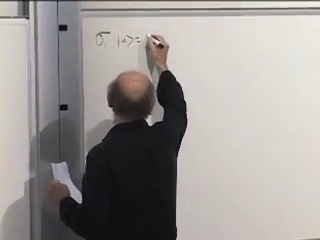
\includegraphics[width=0.62\linewidth]{lecture_05_figure_02.png}
\caption{Die vollständige Tabelle der Pauli-Matrizen-Wirkungen, die im gesamten Vergleich verwendet wird.}
\lectureframe{00:03:15}
\end{figure}

Keiner der beiden Spins hat in einem der Zustände eine bevorzugte Richtung:
\begin{equation}
  \expect{\sigma_i}_{\psi_\pm}=0,
  \qquad
  \expect{\tau_i}_{\psi_\pm}=0,
  \qquad i=1,2,3.
  \label{eq:l05-local-zero}
\end{equation}
Die verlangte explizite Überprüfung für den Pluszustand ergibt zum Beispiel
\begin{align}
  \bra{\psi_+}\sigma_3\ket{\psi_+}
  &=
  \frac12
  \bigl(\bra{ud}+\bra{du}\bigr)
  \bigl(\ket{ud}-\ket{du}\bigr)\nonumber\\
  &=
  \frac12(1-1)=0.
  \label{eq:l05-sigma3-expectation}
\end{align}
Die Kreuzterme verschwinden, weil \(\braket{ud}{du}=0\).

\begin{figure}[htbp]
\centering
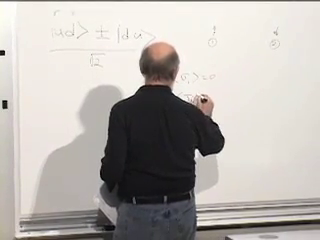
\includegraphics[width=0.78\linewidth]{lecture_05_figure_03.png}
\caption{Der Erwartungswert im Pluszustand wird berechnet, indem man \(\sigma_3\) auf den Zustand wirken lässt und die Orthogonalität verwendet.}
\lectureframe{00:07:00}
\end{figure}

\begin{classroomqa}
\lecturetimestamp{00:07:13}
\audiencequestion{Bedeutet ein Erwartungswert von null, dass man bei einer Einzelmessung am Spin den Wert null erhalten kann?}
\lecturerresponse{Nein. Eine Komponente eines einzelnen Spins kann nur die Werte \(+1\) und \(-1\) annehmen; \(\sigma_i\) hat keinen Eigenwert null. Gleichung~\eqref{eq:l05-local-zero} besagt, dass wiederholte Messungen Ergebnisse wie bei einem fairen Münzwurf liefern, nicht, dass ein einzelnes Ergebnis null ist.}
\end{classroomqa}

Die erste naheliegende Diagnose hat sich also als untauglich erwiesen. Lokale Mittelwerte können das relative Vorzeichen nicht erkennen; daher müssen wir eine Eigenschaft des Teilchenpaars messen.

\section{Der Gesamtspin zeichnet das Singulett aus}

Das magnetische Moment des Paars wird durch die Vektorsumme dargestellt
\begin{equation}
  \boldsymbol{\Sigma}
  =
  \boldsymbol{\sigma}+\boldsymbol{\tau}.
\end{equation}
Ihre dritte Komponente annihiliert beide Basisvektoren:
\begin{align}
  (\sigma_3+\tau_3)\ket{ud}
  &=(1-1)\ket{ud}=0,\nonumber\\
  (\sigma_3+\tau_3)\ket{du}
  &=(-1+1)\ket{du}=0.
\end{align}
Folglich gilt
\begin{equation}
  (\sigma_3+\tau_3)\ket{\psi_\pm}=0.
\end{equation}
Bei beiden Vorzeichen ist die dritte Gesamtspin-Komponente in jedem Versuch null.

Die erste Komponente unterscheidet die beiden Zustände. Aus Gleichung~\eqref{eq:l05-pauli-actions} folgt
\begin{align}
  (\sigma_1+\tau_1)\ket{ud}
  &=\ket{dd}+\ket{uu},\nonumber\\
  (\sigma_1+\tau_1)\ket{du}
  &=\ket{uu}+\ket{dd}.
\end{align}
Also gilt
\begin{align}
  (\sigma_1+\tau_1)\ket{\psi_+}
  &=
  \sqrt2\bigl(\ket{uu}+\ket{dd}\bigr),\nonumber\\
  (\sigma_1+\tau_1)\ket{\psi_-}
  &=0.
  \label{eq:l05-total-x}
\end{align}
Der Pluszustand kann für diese Observable zwar einen Erwartungswert von null haben, ist aber nicht ihr Eigenzustand zum Eigenwert null.

\begin{classroomqa}
\lecturetimestamp{00:13:02}
\audiencequestion{Welche Ergebnisse kann die Gesamtspin-Komponente annehmen, wenn sie den Zustand nicht annihiliert?}
\lecturerresponse{Jedes einzelne Messergebnis ist \(+1\) oder \(-1\), ihre Summe kann also \(2\), \(0\) oder \(-2\) sein. Ein Erwartungswert von null erzwingt nicht, dass das Ergebnis bei jedem Versuch null ist.}
\end{classroomqa}

Die zweite Komponente vervollständigt die Prüfung. Ihre Faktoren \(i\) heben sich in der antisymmetrischen Kombination auf:
\begin{equation}
  (\sigma_2+\tau_2)\ket{\psi_-}=0.
\end{equation}
Damit annihilieren alle drei Komponenten den Minuszustand,
\begin{equation}
  \bigl(\boldsymbol{\sigma}+\boldsymbol{\tau}\bigr)
  \cdot\hat n\,\ket{\psi_-}=0
  \qquad\text{for every unit vector }\hat n.
  \label{eq:l05-singlet-any-axis}
\end{equation}

\begin{figure}[htbp]
\centering
\includegraphics[width=0.84\linewidth]{lecture_05_figure_06.png}
\caption{Die Auslöschungen der einzelnen Komponenten, die den Minuszustand als Zustand mit Gesamtspin null ausweisen.}
\lectureframe{00:16:30}
\end{figure}

Der antisymmetrische Zustand \(\ket{\psi_-}\) ist das \emph{Singulett}. Er ist rotationsinvariant: Bei Messungen entlang jeder Achse ergibt sich derselbe Gesamtspinwert, nämlich null. Der symmetrische Zustand in Gleichung~\eqref{eq:l05-two-signs} gehört zum Triplettsektor.

\begin{classroomqa}
\lecturetimestamp{00:19:06}
\audiencequestion{Gilt das Ergebnis entgegengesetzter Spins nur im Mittel?}
\lecturerresponse{Beim Singulett gilt es bei jedem Versuch. Gleichung~\eqref{eq:l05-singlet-any-axis} ist eine Eigenvektorgleichung. Misst man also an beiden Teilchen dieselbe Komponente, so summieren sich die Ergebnisse stets zum Eigenwert null.}
\end{classroomqa}

\begin{classroomqa}
\lecturetimestamp{00:19:36}
\audiencequestion{Warum heißt der andere Zustand Triplett?}
\lecturerresponse{Der Name geht auf die drei Zustände im Multiplett mit Gesamtspin eins zurück. Die Herleitung folgt später; für die vorliegende Rechnung genügt der Unterschied zwischen dem symmetrischen Zustand und dem eindimensionalen Singulettsektor.}
\end{classroomqa}

Misst Bob eine beliebige Komponente seines Elektrons, weiß er sofort, welches Ergebnis Alice bei einer Messung derselben Komponente an ihrem Elektron erhalten würde: Ihr Ergebnis muss das entgegengesetzte sein. Das ist eine Einstein--Podolsky--Rosen-Korrelation. Ein Paar verborgener Münzen kann ebenfalls entgegengesetzte Ergebnisse tragen, allerdings nur für eine einzige vorab festgelegte Frage. Das Singulett liefert perfekte Antikorrelation für jede gewählte räumliche Achse.

\begin{classroomqa}
\lecturetimestamp{00:20:55}
\audiencequestion{Haben Einstein, Podolsky und Rosen die Verschränkung zuerst entdeckt?}
\lecturerresponse{Nein. Schrödinger erörterte das Phänomen und führte den Begriff der Verschränkung ein. Das EPR-Argument machte das Problem der Korrelationen über große Entfernungen besonders deutlich.}
\end{classroomqa}

\begin{classroomqa}
\lecturetimestamp{00:23:50}
\audiencequestion{Verletzt die unmittelbare Korrelation die Kausalität, und spielt es eine Rolle, welche beobachtende Person zuerst misst?}
\lecturerresponse{Es wird keine nutzbare Nachricht übertragen. Alices lokale Messergebnisse bleiben zu gleichen Teilen verteilt, unabhängig davon, ob Bob misst, und zwar bei jeder zeitlichen Reihenfolge, die mit einem Inertialsystem vereinbar ist. Alice kann die Korrelation erst überprüfen, nachdem sie Bobs Ergebnis über einen gewöhnlichen klassischen Kanal erhalten hat, der sich nicht schneller als Licht ausbreiten kann.}
\end{classroomqa}

\section{Bells Ungleichung ist klassische Zählung}

Der Stellenwert von Bells Ergebnis kann wechselhaft erscheinen. An manchen Tagen wirkt es wie das tiefste Merkmal der Quantenmechanik, an anderen wie eine weitere unvermeidliche Konsequenz des Formalismus. Sowohl Bell selbst als auch Feynman konnten beide Sichtweisen vertreten. Die Ungleichung ist jedoch elementar. Die Überraschung liegt in ihrer Verletzung.

Betrachten wir eine gewöhnliche Menge von Objekten. Jedes Objekt kann die drei Eigenschaften \(A\), \(B\) und \(C\) besitzen oder nicht. \(N(A,\neg B)\) bezeichne die Anzahl der Objekte, die \(A\), aber nicht \(B\) besitzen. Die klassische Mengenlogik impliziert
\begin{equation}
  N(A,\neg B)+N(B,\neg C)
  \geq
  N(A,\neg C).
  \label{eq:l05-bell-count}
\end{equation}
Der Beweis folgt aus der Mengeninklusion
\begin{equation}
  A\cap C^{c}
  \subseteq
  (A\cap B^{c})\cup(B\cap C^{c}).
  \label{eq:l05-set-inclusion}
\end{equation}
Tatsächlich gehört ein Element von \(A\cap C^c\) entweder zu \(B\) oder nicht. Im ersten Fall gehört es zu \(B\cap C^c\), im zweiten zu \(A\cap B^c\). Beim Zählen der Vereinigung können daher nur zusätzliche Elemente zur Menge auf der linken Seite hinzukommen.

\begin{figure}[htbp]
\centering
\includegraphics[width=0.78\linewidth]{lecture_05_figure_07.png}
\caption{Der Tafelbeweis zerlegt drei sich überschneidende klassische Teilmengen in Bereiche mit nichtnegativen Anzahlen.}
\lectureframe{00:31:15}
\end{figure}

Äquivalent dazu kann man die disjunkten Bereiche des Diagramms der drei Mengen mit nichtnegativen ganzen Zahlen \(N_i\) beschriften. Beide Seiten von Gleichung~\eqref{eq:l05-bell-count} enthalten die für \(A\cap C^c\) erforderlichen Bereiche, während die linke Seite zusätzliche Bereiche mit nichtnegativen Anzahlen enthält. Hier kommt nichts Quantenmechanisches vor. Es handelt sich um einen Satz über Teilmengen und gewöhnliche logische Alternativen.

\section{Die Mengenaussage in ein Spinexperiment übertragen}

Wir präparieren viele unabhängige Elektronenpaare im Singulettzustand und definieren drei Aussagen über Elektron 1:
\begin{align}
  A&:\ \text{spin 1 is up at }0^\circ\text{, along the third axis},\nonumber\\
  B&:\ \text{spin 1 is up at }45^\circ\text{ in the }zx\text{-plane},\nonumber\\
  C&:\ \text{spin 1 is up at }90^\circ\text{, along the first axis}.
  \label{eq:l05-abc}
\end{align}

\begin{figure}[htbp]
\centering
\includegraphics[width=0.82\linewidth]{lecture_05_figure_08.png}
\caption{Die drei Spin-Aussagen beziehen sich auf die Richtungen \(0^\circ\), \(45^\circ\) und \(90^\circ\) in einer Ebene.}
\lectureframe{00:39:00}
\end{figure}

Im Singulett lässt sich die Negation einer Aussage über Elektron 1 als positive Aussage über Elektron 2 umformulieren. Zum Beispiel gilt
\begin{align}
  \neg B
  &:\ \text{spin 1 is down at }45^\circ\nonumber\\
  &\Longleftrightarrow
  \text{spin 2 is up at }45^\circ.
\end{align}
Entsprechend wird aus \(\neg C\) die Aussage, dass Elektron 2 bei \(90^\circ\) spinaufwärts ist.

\begin{classroomqa}
\lecturetimestamp{00:40:04}
\audiencequestion{Sollte \(\neg C\) bedeuten, dass Elektron 2 bei \(90^\circ\) spinabwärts ist?}
\lecturerresponse{Nein. Negiere zuerst \(C\): Elektron 1 ist bei \(90^\circ\) spinabwärts. Die perfekte Antikorrelation des Singuletts bedeutet dann, dass Elektron 2 entlang derselben Achse spinaufwärts ist. Die beiden Umkehrungen müssen getrennt behandelt werden.}
\end{classroomqa}

Für ein großes Ensemble unterscheiden sich Anzahlen und Wahrscheinlichkeiten nur durch die gemeinsame Zahl der präparierten Paare. Rotationsinvarianz ergibt außerdem
\begin{equation}
  P(A,\neg B)=P(B,\neg C),
\end{equation}
denn das zweite Experiment entsteht durch eine Drehung des ersten um \(45^\circ\). Bells klassische Ungleichung würde daher verlangen,
\begin{equation}
  2P(A,\neg B)\geq P(A,\neg C).
  \label{eq:l05-bell-probability}
\end{equation}
Nun benötigen wir eine effiziente Methode, diese Wahrscheinlichkeiten zu berechnen.

\section{Aussagen werden zu Projektoren}

In einem gewöhnlichen dreidimensionalen Vektorraum entfernt ein Projektor alle Komponenten, die senkrecht auf einem gewählten Unterraum stehen. Ein eindimensionaler Projektor projiziert einen Vektor orthogonal auf eine Gerade, ein zweidimensionaler auf eine Ebene. Wenn \(P\) auf einen bestimmten Unterraum projiziert, gilt
\begin{equation}
  P\ket{\alpha}=\ket{\alpha_P}.
\end{equation}

\begin{figure}[htbp]
\centering
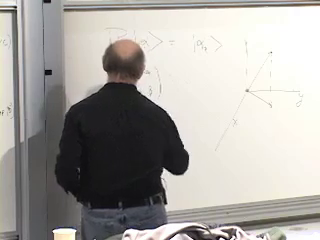
\includegraphics[width=0.76\linewidth]{lecture_05_figure_04.png}
\caption{Geometrische Projektion und Operatornotation werden parallel zueinander eingeführt.}
\lectureframe{00:49:53}
\end{figure}

\begin{figure}[htbp]
\centering
\begin{tikzpicture}[scale=1.05,>=Latex]
  \draw[->] (-0.25,0)--(4.0,0);
  \draw[thick] (-0.25,-0.25)--(3.55,2.6);
  \draw[->,very thick] (0,0)--(2.25,3.05)
    node[above] {\(\ket{\alpha}\)};
  \coordinate (P) at (2.72,1.98);
  \draw[dashed] (2.25,3.05)--(P);
  \draw[->,very thick] (0,0)--(P)
    node[right] {\(\ket{\alpha_P}\)};
  \node[below right] at (3.1,2.25) {projected subspace};
\end{tikzpicture}
\caption{Eine klare Rekonstruktion der Projektionsgeometrie.}
\end{figure}

Im Hilbertraum eines Spins entspricht die Aussage, dass \(\sigma_3=+1\), dem eindimensionalen Unterraum, der von \(\ket{u}\) aufgespannt wird. Der zugehörige Projektor wirkt folgendermaßen:
\begin{equation}
  P_{\sigma_3=+1}
  \begin{pmatrix}\alpha\\\beta\end{pmatrix}
  =
  \begin{pmatrix}\alpha\\0\end{pmatrix},
  \qquad
  P_{\sigma_3=-1}
  \begin{pmatrix}\alpha\\\beta\end{pmatrix}
  =
  \begin{pmatrix}0\\\beta\end{pmatrix}.
  \label{eq:l05-projector-actions}
\end{equation}

\begin{classroomqa}
\lecturetimestamp{00:49:55}
\audiencequestion{Gibt der erste Projektor an, wie hoch der Vektor auf einer vertikalen Achse reicht?}
\lecturerresponse{Nein. Er verwirft einfach den orthogonalen Koeffizienten \(\beta\). Bei den Komponenten handelt es sich um Amplituden im Hilbertraum, nicht um gewöhnliche räumliche Koordinaten des Spins.}
\end{classroomqa}

\begin{figure}[htbp]
\centering
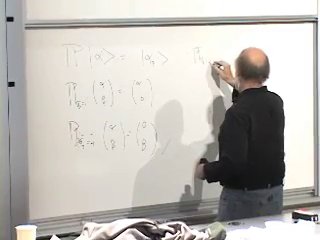
\includegraphics[width=0.78\linewidth]{lecture_05_figure_05.png}
\caption{Zuerst wirken die Projektoren auf einen allgemeinen Spinor, anschließend werden sie als explizite Matrizen angegeben.}
\lectureframe{00:51:40}
\end{figure}

Die Matrixdarstellung lautet
\begin{equation}
  P_{\sigma_3=+1}
  =
  \begin{pmatrix}1&0\\0&0\end{pmatrix}
  =
  \frac{I+\sigma_3}{2}.
  \label{eq:l05-p3}
\end{equation}
Dieselbe Konstruktion gilt für jeden Einheitsvektor \(\hat n\):
\begin{equation}
  P_{\boldsymbol{\sigma}\cdot\hat n=+1}
  =
  \frac{I+\boldsymbol{\sigma}\cdot\hat n}{2}.
  \label{eq:l05-pn}
\end{equation}

\begin{classroomqa}
\lecturetimestamp{00:53:09}
\audiencequestion{Wie lautet der Projektor auf \(\sigma_1=+1\)?}
\lecturerresponse{Ersetze \(\sigma_3\) in Gleichung~\eqref{eq:l05-p3} durch \(\sigma_1\): \(P_{\sigma_1=+1}=(I+\sigma_1)/2\).}
\end{classroomqa}

Die Bornsche Regel lässt sich nun in einer nützlichen Form für Aussagen formulieren:
\begin{equation}
  P(\mathcal A\text{ is true in }\ket{\psi})
  =
  \bra{\psi}P_{\mathcal A}\ket{\psi}.
  \label{eq:l05-projector-born}
\end{equation}
Für einen normierten Spinor \(\ket{\psi}=(\alpha,\beta)^T\) ergibt Gleichung~\eqref{eq:l05-projector-born} mit \(P_{\sigma_3=+1}\) den Wert \(|\alpha|^2\), genau wie erwartet.

Diese Sprache macht den Unterschied zwischen klassischen und quantenmechanischen Aussagen deutlich. In der klassischen Logik entspricht eine Eigenschaft einer Teilmenge einer Menge. In der Quantenmechanik entspricht eine Eigenschaft einem Unterraum des Hilbertraums oder gleichbedeutend dem zugehörigen Projektor. Teilmengen und Vektorunterräume erfüllen nicht dieselben Verbandsgesetze; aus diesem Unterschied erwächst Bells Widerspruch.

\subsection{Der gemeinsame Bell-Projektor}

Für \(A\wedge\neg B\) muss Elektron 1 entlang der dritten Achse spinaufwärts sein und Elektron 2 entlang
\begin{equation}
  \hat n_{45}=\frac{\hat x+\hat z}{\sqrt2}.
\end{equation}
Die betreffende Komponente des zweiten Spins lautet
\begin{equation}
  \boldsymbol{\tau}\cdot\hat n_{45}
  =
  \frac{\tau_1+\tau_3}{\sqrt2}.
\end{equation}
Der gemeinsame Projektor ist daher
\begin{equation}
  P_{A\wedge\neg B}
  =
  \frac{I+\sigma_3}{2}
  \frac{I+(\tau_1+\tau_3)/\sqrt2}{2}.
  \label{eq:l05-joint-projector}
\end{equation}

\begin{classroomqa}
\lecturetimestamp{00:59:18}
\audiencequestion{Warum steht in der Spin-Komponente bei \(45^\circ\) ein Faktor \(1/\sqrt2\)?}
\lecturerresponse{Die Richtung muss ein Einheitsvektor sein. Ihre Komponenten entlang der ersten und dritten Achse betragen jeweils \(1/\sqrt2\); die zugehörige Observable lautet daher \((\tau_1+\tau_3)/\sqrt2\).}
\end{classroomqa}

\begin{classroomqa}
\lecturetimestamp{01:00:52}
\audiencequestion{Wird der gesamte Ausdruck \(I+\boldsymbol{\tau}\cdot\hat n_{45}\) durch zwei geteilt?}
\lecturerresponse{Ja. Der Projektor lautet \(\bigl(I+\boldsymbol{\tau}\cdot\hat n_{45}\bigr)/2\); der Faktor \(1/2\) multipliziert den gesamten Zähler.}
\end{classroomqa}

Die beiden Faktoren in Gleichung~\eqref{eq:l05-joint-projector} wirken auf verschiedene Tensorfaktoren und kommutieren. Wendet man beide nacheinander an, werden zuerst alle Komponenten mit Elektron 1 im Spin-abwärts-Zustand entfernt, dann alle verbleibenden Komponenten, in denen Elektron 2 entlang \(\hat n_{45}\) spinabwärts ist.

\section{Die Quantenzahlen kehren die Ungleichung um}

Sei
\begin{equation}
  \ket{\psi_s}
  =
  \frac{\ket{ud}-\ket{du}}{\sqrt2}
\end{equation}
das Singulett. Wir beginnen mit
\begin{equation}
  P(A,\neg B)
  =
  \bra{\psi_s}P_{A\wedge\neg B}\ket{\psi_s}.
\end{equation}
Der Faktor \((I+\sigma_3)/2\) vernichtet \(\ket{du}\) und lässt \(\ket{ud}/\sqrt2\) übrig. Der zweite Faktor ergibt dann
\begin{align}
  \frac{I+(\tau_1+\tau_3)/\sqrt2}{2}\ket{ud}
  &\notag\\[-0.3em]
  &=
  \frac12
  \left[
    \ket{ud}
    +\frac{\ket{uu}-\ket{ud}}{\sqrt2}
  \right]\nonumber\\
  &=
  \frac12
  \Biggl[
    \left(1-\frac1{\sqrt2}\right)\ket{ud}
  \nonumber\\
  &\qquad
    +\frac1{\sqrt2}\ket{uu}\Biggr].
  \label{eq:l05-projector-action}
\end{align}
Der Term \(\ket{uu}\) hat mit dem Singulett-Bra die Überlappung null, und die verbleibenden Normierungsfaktoren ergeben
\begin{equation}
  P(A,\neg B)
  =
  \frac14\left(1-\frac1{\sqrt2}\right).
  \label{eq:l05-pab}
\end{equation}

\begin{figure}[htbp]
\centering
\includegraphics[width=0.88\linewidth]{lecture_05_figure_09.png}
\caption{Bei der Projektorrechnung wird die Überlappung mit \(\ket{ud}\) berücksichtigt und der orthogonale Beitrag \(\ket{uu}\) verworfen.}
\lectureframe{01:08:20}
\end{figure}

Rotationsinvarianz liefert dasselbe Ergebnis für das nächste Richtungspaar:
\begin{equation}
  P(B,\neg C)
  =
  \frac14\left(1-\frac1{\sqrt2}\right).
\end{equation}
Für \(A\wedge\neg C\) liegt die zweite Achse entlang der ersten räumlichen Achse, also gilt
\begin{equation}
  P_{A\wedge\neg C}
  =
  \frac{I+\sigma_3}{2}\frac{I+\tau_1}{2}.
\end{equation}
Der erste Faktor lässt erneut \(\ket{ud}/\sqrt2\) übrig. Der Term \(\tau_1\) ergibt \(\ket{uu}\), das zum Singulett-Bra orthogonal ist; der Identitätsterm bleibt dagegen erhalten. Somit gilt
\begin{equation}
  P(A,\neg C)=\frac14.
  \label{eq:l05-pac}
\end{equation}
Fasst man die drei Ergebnisse zusammen, erhält man
\begin{equation}
  \underbrace{
  P(A,\neg B)+P(B,\neg C)
  }_{\frac12(1-1/\sqrt2)\approx0.146}
  <
  \underbrace{
  P(A,\neg C)
  }_{\frac14=0.25}.
  \label{eq:l05-bell-violation}
\end{equation}

\begin{figure}[htbp]
\centering
\includegraphics[width=0.84\linewidth]{lecture_05_figure_10.png}
\caption{Die vollständige Tafelrechnung zeigt, dass die linke Seite der Bell-Ungleichung kleiner ist als die rechte.}
\lectureframe{01:12:15}
\end{figure}

Gleichung~\eqref{eq:l05-bell-violation} kehrt Gleichung~\eqref{eq:l05-bell-probability} um. Daraus folgt nicht, dass die Quantenmechanik sich widerspricht. Vielmehr können die Korrelationen des Singuletts nicht aus einem lokalen klassischen Modell hervorgehen, in dem alle drei Spin-Aussagen unabhängig von der entfernten Messwahl gewöhnliche Wahrheitswerte im mengentheoretischen Sinn besitzen. Eine klassische Simulation kann die Korrelationen nur reproduzieren, wenn sie mindestens eine Bell-Annahme aufgibt; am deutlichsten zeigt sich das bei der Lokalität.

\section{Was das Bell-Experiment prüft}

Die Quantenmechanik sagt die Verletzung bereits voraus. Ein Experiment muss zusätzlich den klassischen Ausweg ausschließen, bei dem ein Detektor dem anderen mitteilt, welche Einstellung oder welches Ergebnis er vorgefunden hat. Die beiden Seiten müssen weit genug voneinander entfernt sein, und Wahl der Einstellungen sowie Detektion müssen zeitlich so dicht aufeinander folgen, dass ein Signal mit Lichtgeschwindigkeit nicht zwischen ihnen übertragen werden kann. Aspects Experiment machte diese zeitliche Abstimmung und Abschirmung auf überzeugende Weise praktisch umsetzbar.

\begin{classroomqa}
\lecturetimestamp{01:13:15}
\audiencequestion{Haben uns die Bell-Experimente etwas gelehrt, wenn die Quantenmechanik das Ergebnis bereits vorhersagt?}
\lecturerresponse{Sie prüften, ob die Natur bei genau diesem Korrelationsexperiment der quantenmechanischen Vorhersage folgt, und sorgten vor allem dafür, dass die beiden Messstationen während der maßgeblichen Lichtlaufzeit unabhängig voneinander waren. Die experimentelle Kontrolle und die zeitliche Abstimmung waren selbst bedeutende Leistungen.}
\end{classroomqa}

\begin{classroomqa}
\lecturetimestamp{01:18:19}
\audiencequestion{Was fügte Bell der Diskussion Einsteins über die spukhafte Fernwirkung hinzu?}
\lecturerresponse{Bell lieferte eine quantitative Ungleichung. Er zeigte ein durchführbares Korrelationsexperiment auf, dessen quantenmechanische Vorhersage eine lokale klassische Erklärung der zugrunde liegenden Vorgänge ausschließt. Damit blieb der Einwand nicht bei philosophischem Unbehagen stehen. Bell blieb zwiespältig, ob dies unvermeidlich oder tiefgreifend sei, und stellte die Standard-Quantenmechanik zunehmend infrage.}
\end{classroomqa}

Die Teilchen können kilometerweit voneinander entfernt sein und dennoch einen gemeinsamen Zustand teilen; trotzdem handelt es sich um ein Quantenexperiment mit kleinen Systemen. Wechselwirkungen mit der Umgebung zerstören leicht die erforderlichen Phasenbeziehungen. Luftmoleküle, Streuphotonen und thermische Störungen können sich mit dem Paar verschränken. Deshalb muss die Trennung in einer kalten, gut abgeschirmten Umgebung erfolgen.

\begin{classroomqa}
\lecturetimestamp{01:19:53}
\audiencequestion{Macht ein gemeinsamer Zustand, der sich über eine große Entfernung erstreckt, daraus ein makroskopisches Quantenobjekt?}
\lecturerresponse{Treffender ist die Beschreibung als weit voneinander entfernte kleine Quantensysteme. Ihr Abstand kann groß sein, doch die gemeinsame Wellenfunktion zu erhalten wird immer heikler, weil unkontrollierte Wechselwirkungen mit der Umgebung die nutzbare Kohärenz zerstören. Zwei gewöhnliche Bowlingkugeln ergeben nicht dasselbe Experiment.}
\end{classroomqa}

\begin{classroomqa}
\lecturetimestamp{01:21:23}
\audiencequestion{Kann eine Messung an einem Teilchen komplementäre Informationen über das andere offenbaren und so die Unschärferelation umgehen?}
\lecturerresponse{Man kann zum Beispiel die Position des einen Teilchens und den Impuls des anderen messen. Das ist keine gleichzeitige Messung nichtkommutierender Observablen an einem Teilchen. Die Unschärferelation für ein einzelnes System wird dadurch nicht umgangen.}
\end{classroomqa}

\section{Wann bedeutet ein Produkt »und«?}

In der Bell-Rechnung wurden zwei Projektoren miteinander multipliziert. Das stellt eine Konjunktion nur für miteinander verträgliche Aussagen dar.

\begin{classroomqa}
\lecturetimestamp{01:22:39}
\audiencequestion{Warum stellte das Produkt zweier Projektoren das logische Wort »und« dar?}
\lecturerresponse{Weil die beiden Projektoren kommutieren. Einer wirkt auf Elektron 1, der andere auf Elektron 2; ihre Reihenfolge spielt also keine Rolle, und beide Eigenschaften können gemeinsam geprüft werden. Für ein einzelnes Elektron kommutieren \((I+\sigma_3)/2\) und \((I+\sigma_1)/2\) nicht; Spinaufwärts entlang beider Achsen ist keine gemeinsam bestimmte Aussage dieser Art.}
\end{classroomqa}

Hier zeigt sich erneut, dass quantenmechanische Aussagen von gewöhnlichen Teilmengen abweichen. Ein klassischer Schnitt existiert immer. Das quantenmechanische Gegenstück, das durch ein Produkt von Projektoren dargestellt wird, hat die beabsichtigte logische Bedeutung nur, wenn die betreffenden Unterräume miteinander verträglich sind.

Dieselbe Diskussion führt zur Messung selbst. Ein Messgerät besitzt einen Zeigerzustand. Wenn ein Spin-aufwärts-Elektron den Zeiger in die eine Richtung bewegt und ein Spin-abwärts-Elektron in die andere, verschränkt sich ein Elektron in einer Superposition mit zwei Zeigerpositionen. Messung lässt sich daher als Verschränkung zwischen System und Messapparat untersuchen. Diese Frage stellen wir zurück und wenden uns einem kürzeren Satz zu, der nur die Linearität voraussetzt.

\begin{classroomqa}
\lecturetimestamp{01:25:09}
\audiencequestion{Lässt sich der Kollaps der Wellenfunktion sinnvoll als eine Messung auffassen, die den gemeinsamen Zustand einschränkt?}
\lecturerresponse{Diese Frage gehört zum Messprozess. Messapparat und gemessenes System verschränken sich: Ein Spinwert korreliert mit einer Zeigerposition, der andere mit einer anderen. Die ausführliche Diskussion der Messung folgt später.}
\end{classroomqa}

\section{Die Linearität verbietet eine universelle Xeroxmaschine}

Für die zeitliche Entwicklung benötigen wir nur eine einzige Tatsache. Wenn ein physikalischer Prozess abbildet
\begin{equation}
  \ket{a}\longrightarrow\ket{a'},
  \qquad
  \ket{b}\longrightarrow\ket{b'},
\end{equation}
verlangt die Linearität
\begin{equation}
  \alpha\ket{a}+\beta\ket{b}
  \longrightarrow
  \alpha\ket{a'}+\beta\ket{b'}.
  \label{eq:l05-linearity}
\end{equation}

Eine gewöhnliche Kopiermaschine kann klassische Informationen mit kontrollierbar kleinen Fehlern vervielfältigen. Die quantenmechanische Forderung ist stärker: Ein einziges festgelegtes Gerät muss sämtliche Amplituden eines beliebigen ihm zugeführten Zustands duplizieren. Deshalb wird das No-Cloning-Theorem auch als No-Quantum-Xerox-Prinzip bezeichnet.

Man stelle sich eine Maschine mit einem Eingang und zwei Ausgängen vor. Wenn sie die Basiszustände entlang der dritten Achse klont, muss sie folgende Abbildung ausführen:
\begin{equation}
  \ket{u}\longrightarrow\ket{uu},
  \qquad
  \ket{d}\longrightarrow\ket{dd}.
  \label{eq:l05-clone-basis}
\end{equation}
Die Maschine darf ihren Ausgängen Energie, Masse oder Ladung zuführen; die Erhaltungssätze sind nicht das Hindernis. Der Widerspruch betrifft die Zustandsabhängigkeit der Transformation.

\begin{figure}[H]
\centering
\includegraphics[width=0.86\linewidth]{lecture_05_figure_11.png}
\caption{Von einer hypothetischen Maschine mit einem Eingang und zwei Ausgängen wird verlangt, beide Basiszustände zu duplizieren.}
\lectureframe{01:33:45}
\end{figure}

Nun präparieren wir einen Spin, der nach rechts zeigt:
\begin{equation}
  \ket{r}
  =
  \frac{\ket{u}+\ket{d}}{\sqrt2}.
  \label{eq:l05-right-state}
\end{equation}
Gleichungen~\eqref{eq:l05-linearity} und \eqref{eq:l05-clone-basis} erzwingen als Ausgabe
\begin{equation}
  \ket{r}
  \longrightarrow
  \frac{\ket{uu}+\ket{dd}}{\sqrt2}.
  \label{eq:l05-linear-output}
\end{equation}
Exaktes Klonen verlangt stattdessen zwei unabhängige Kopien:
\begin{align}
  \ket{rr}
  &=
  \ket{r}\otimes\ket{r}\nonumber\\
  &=
  \frac12
  \left(
    \ket{uu}+\ket{ud}+\ket{du}+\ket{dd}
  \right).
  \label{eq:l05-cloned-output}
\end{align}
Die gemischten Terme in Gleichung~\eqref{eq:l05-cloned-output} fehlen in Gleichung~\eqref{eq:l05-linear-output}. Die beiden Ausgaben sind verschieden.

\begin{figure}[H]
\centering
\includegraphics[width=0.72\linewidth]{lecture_05_figure_12.png}
\caption{Die Linearität liefert nur die Terme mit parallelen Spins, während zwei echte Kopien des nach rechts zeigenden Spins auch beide gemischten Terme enthalten.}
\lectureframe{01:35:20}
\end{figure}

\begin{theorem}[No-cloning]
Keine einzelne physikalische Maschine kann jeden unbekannten Quantenzustand exakt klonen.
\end{theorem}

\begin{proof}
Angenommen, eine Maschine klont die orthogonalen Basiszustände wie in Gleichung~\eqref{eq:l05-clone-basis}. Die Linearität legt dann ihre Ausgabe für die Superposition gemäß Gleichung~\eqref{eq:l05-linear-output} fest. Exaktes Klonen desselben Eingangszustands verlangt Gleichung~\eqref{eq:l05-cloned-output}. Da sich die beiden Zustandsvektoren unterscheiden, kann die angenommene universelle Maschine nicht existieren.
\end{proof}

Der Grund ist struktureller Art. Die Abbildung von \(\ket{\psi}\) auf \(\ket{\psi}\otimes\ket{\psi}\) hängt quadratisch von den Amplituden ab, während jede zulässige Entwicklung des vollständigen Quantenzustands linear ist.

\begin{classroomqa}
\lecturetimestamp{01:35:49}
\audiencequestion{Setzt der Beweis voraus, dass die beiden Ausgaben unabhängig sind?}
\lecturerresponse{Ja, denn zwei Klone müssen unabhängig voneinander nutzbare Kopien sein. Unabhängige Systeme werden durch das Tensorprodukt kombiniert; deshalb lauten zwei Kopien des nach rechts zeigenden Zustands \(\ket{r}\otimes\ket{r}\). Korrelierte Ausgaben, die sich nicht getrennt verwenden lassen, sind keine zwei Klone.}
\end{classroomqa}

\begin{classroomqa}
\lecturetimestamp{01:37:20}
\audiencequestion{Ein Laser scheint durch stimulierte Emission den Zustand eines Photons zu kopieren. Wo scheitert das Argument?}
\lecturerresponse{Auch das Atom und die elektromagnetischen Moden sind beteiligt. Ihr Zustand trägt zur Ausgabe bei und erscheint aus Sicht des universellen Klonens als Rauschen. Näherungsweises Klonen ist möglich, perfektes, zustandsunabhängiges Klonen dagegen nicht.}
\end{classroomqa}

\begin{classroomqa}
\lecturetimestamp{01:40:24}
\audiencequestion{Kann Quanteninformation übertragen werden, obwohl sie nicht vervielfältigt werden kann?}
\lecturerresponse{Ja. Übertragung ist ein anderer Vorgang: Der ursprüngliche Träger muss den Zustand nicht behalten. Das No-Cloning-Theorem verbietet es, am Ende zwei unabhängige perfekte Kopien zu besitzen, nicht aber, den Zustand von einem Träger auf einen anderen zu übertragen.}
\end{classroomqa}

\begin{classroomqa}
\lecturetimestamp{01:41:03}
\audiencequestion{Muss der Eingangszustand unbekannt sein?}
\lecturerresponse{Ist ein Zustand im Voraus bekannt, kann man weitere Systeme in diesem Zustand präparieren oder ein Gerät bauen, das auf eine gewählte orthogonale Basis zugeschnitten ist. Unmöglich ist eine einzige Maschine, die einen beliebigen Eingang annimmt und ihn ohne vorherige Kenntnis des eingetroffenen Zustands dupliziert.}
\end{classroomqa}

\begin{classroomqa}
\lecturetimestamp{01:42:35}
\audiencequestion{Welcher der beiden Ausdrücke für den Zustand nach rechts beschreibt die tatsächliche Maschinenausgabe?}
\lecturerresponse{Die Linearität erzwingt Gleichung~\eqref{eq:l05-linear-output}; das Klonen verlangt Gleichung~\eqref{eq:l05-cloned-output}. Ihre Abweichung ist genau der Widerspruch.}
\end{classroomqa}

\begin{classroomqa}
\lecturetimestamp{01:43:40}
\audiencequestion{Lässt sich die zusätzliche Information quantifizieren, die verschränkte Zweiteilchenzustände tragen?}
\lecturerresponse{Ein reiner Zustand eines einzelnen Spins hat zwei reelle physikalische Parameter. Zwei getrennt präparierte Spins liefern vier, während ein allgemeiner reiner Zustand im vierdimensionalen Hilbertraum zweier Spins nach Abzug der Normierungsbedingung und der Gesamtphase sechs Parameter hat. Zu den zusätzlichen Zuständen zählen verschränkte Zustände; ihr Verschränkungsgrad lässt sich durch die Verschränkungsentropie quantifizieren.}
\end{classroomqa}

\enlargethispage{4\baselineskip}Das Vorzeichen in Gleichung~\eqref{eq:l05-two-signs} hat nun drei Aufgaben erfüllt. Es wählte den eindeutigen Zustand mit Gesamtspin null aus, lieferte Korrelationen, die eine klassische Mengenungleichung verletzen, und machte den Unterschied zwischen einer linearen quantenmechanischen Entwicklung und dem nichtlinearen Vorgang des Erzeugens zweier Kopien deutlich. Jedes dieser Ergebnisse folgt daraus, dass wir den gemeinsamen Zustand als Vektor im vollständigen Tensorproduktraum behandeln und nicht als Liste bereits vorhandener lokaler Eigenschaften.
